
\begin{document}

\chapter{Testing}

\label{chapter:testing}

The system running multiple Kinects is verified by looking at the skeleton visualization on the user interface for a number of different users and in various interaction scenarios. The researcher is interested in whether the application has accomplished the following tasks:

\begin{enumerate}
  \item The skeletons from different Kinect fields of view are matched correctly to the corresponding persons in the scene.
  \item The transformed skeletons of the same person are close together, showing minimal differences in the joint coordinates.
  \item The skeletons can be transformed to different Kinects' Camera Space (3D coordinate system) for viewing
  \item All of the above statements hold when the users move freely.
\end{enumerate}

\section{Tracking}

Figure~\ref{fig:tracking_disjoined_views}

\begin{figure}[!h]
  \centering
  
  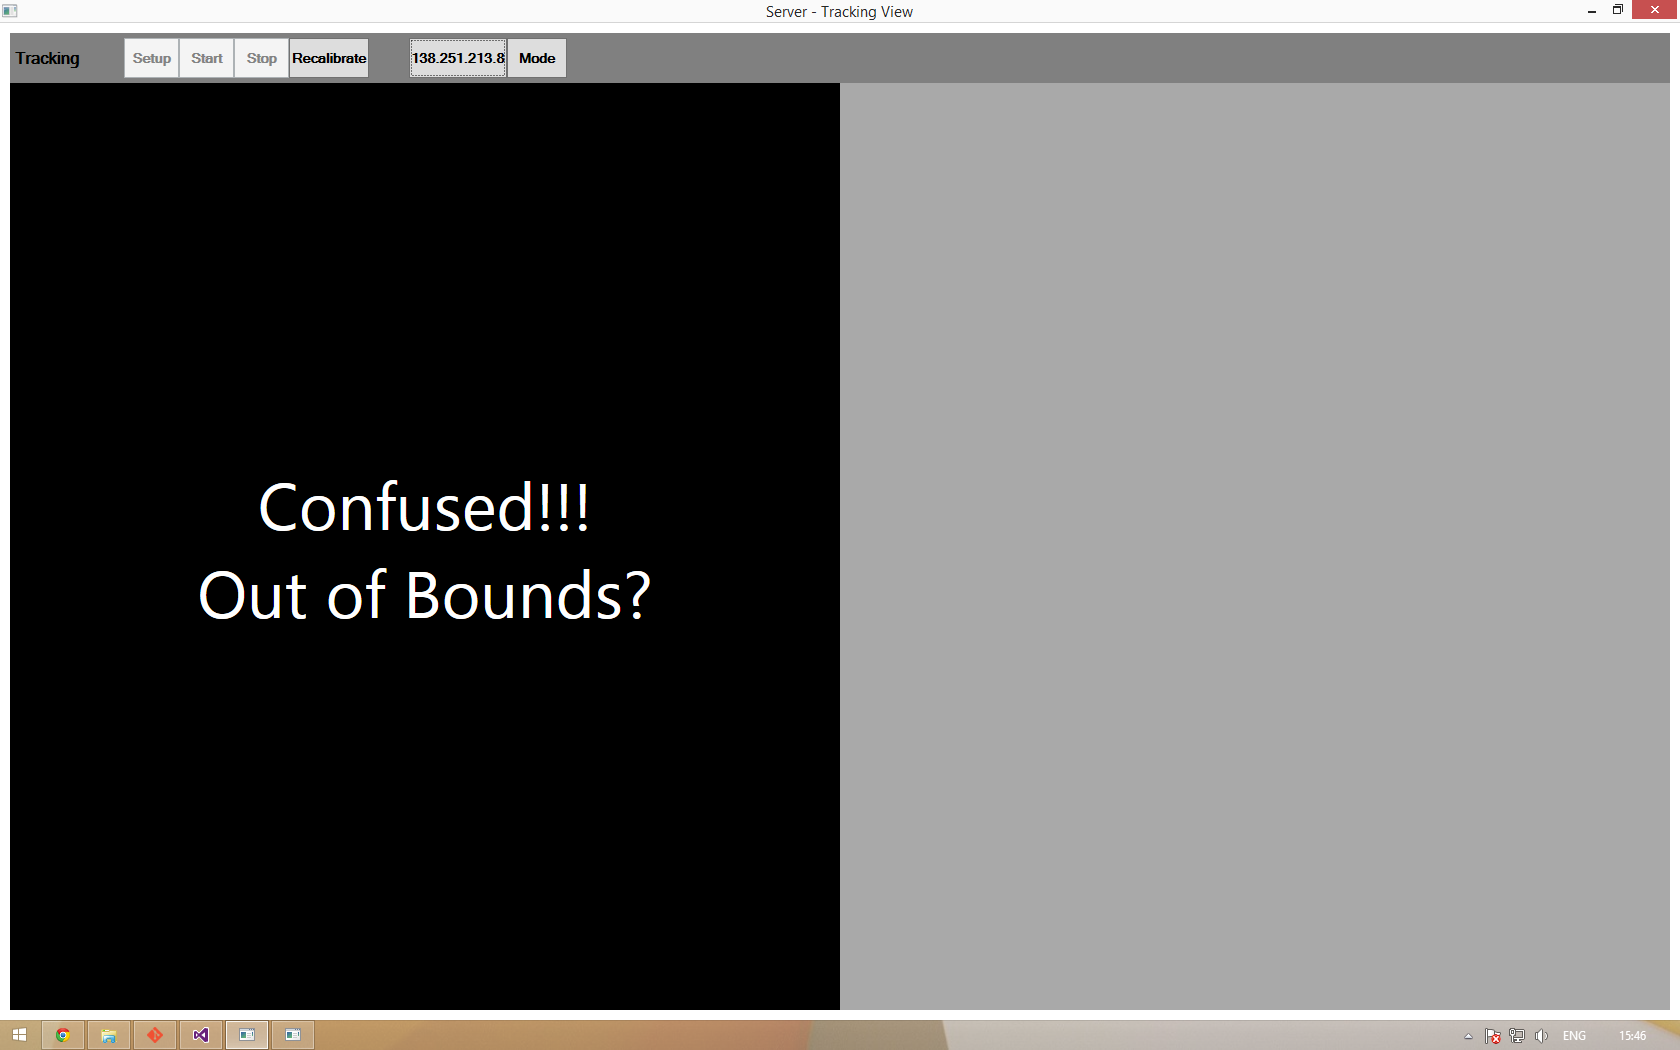
\includegraphics[width=0.5\linewidth]{figs/confused}

  \caption{User interface showing a reminder when the tracker detects people have disappeared.}
  
  \label{fig:tracking_confused}
\end{figure}

\section{Occlusion}

The main goal of the project is to show persistent tracking results in occluded environments and scenarios where complex human interactions are in play. The researcher has verified this requirement by partially and fully obstructing users in the scene. In the simplest case, a person may be self-occluded if he stands in a position such that one Kinect cannot fully see all the joints but two Kinects combined can have a complete view of the person. \textbf{(todo: show an illustration)} The research stands back-facing the main Kinect, while showing his right arm only to the second Kinect. The system would form the average skeleton using the actively tracked information from both Kinects; the average skeleton would contain joint coordinates that both Kinects are most sure about.


\begin{figure}[!h]
  \centering
  \subfloat[The skeletons when the person is visible to both Kinects]{
    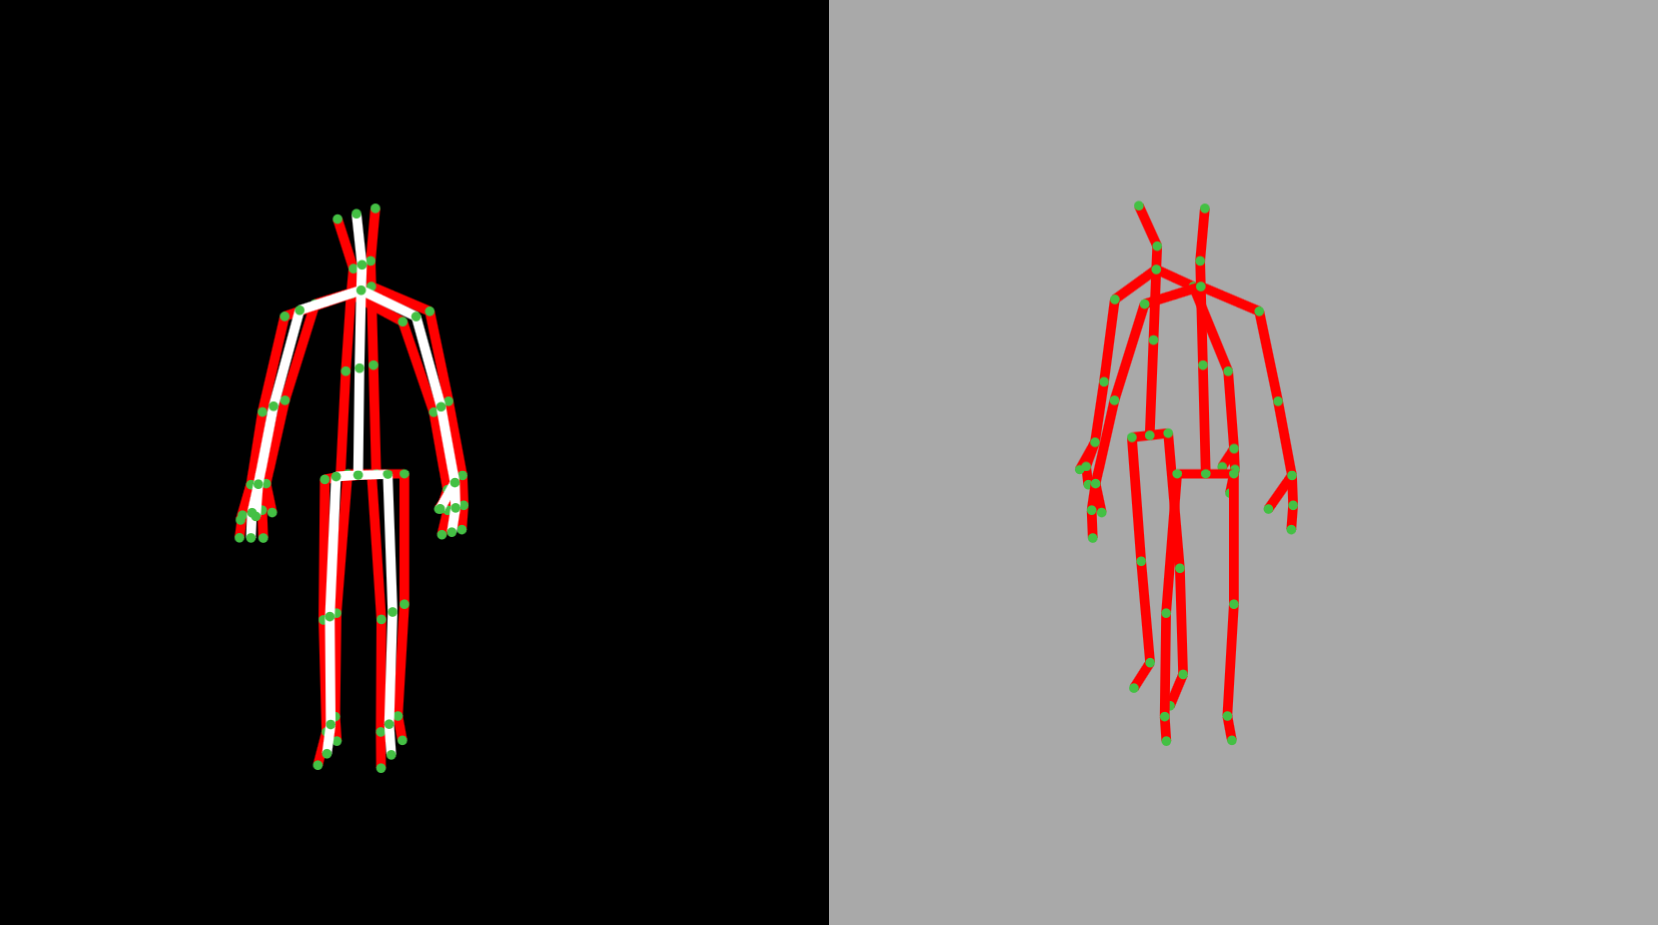
\includegraphics[width=0.5\linewidth]{figs/fill_in_gaps_before}
  }
  \subfloat[The skeletons when the person is self-occluded]{
    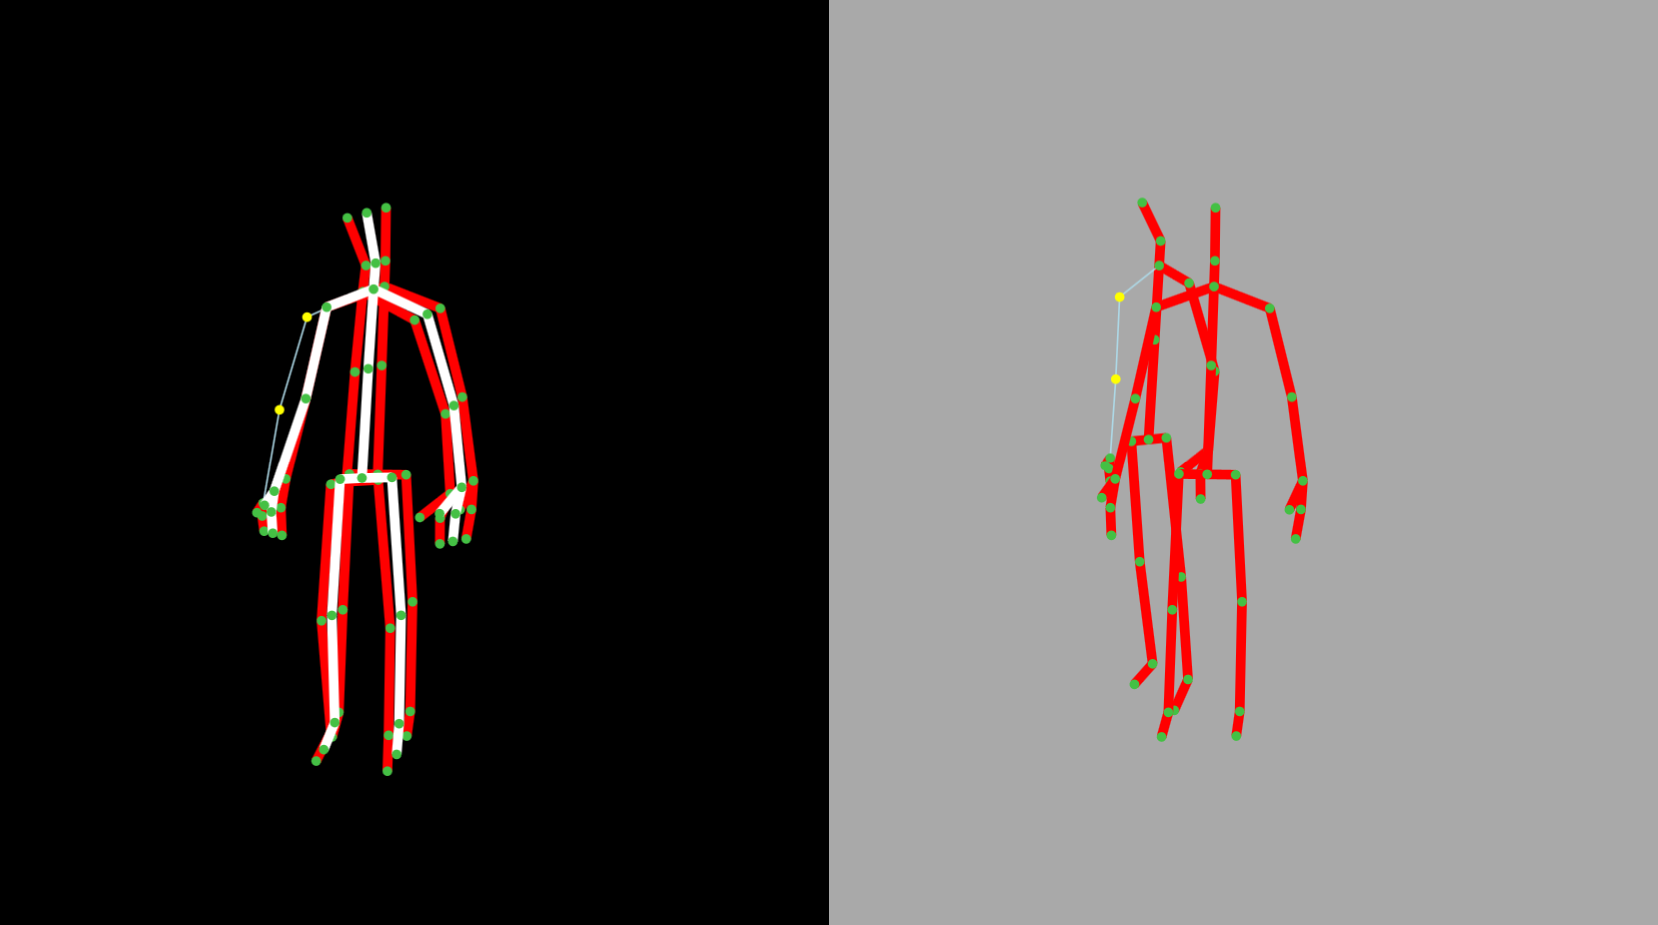
\includegraphics[width=0.5\linewidth]{figs/fill_in_gaps_after}
  }

  \caption{Skeleton visualization showing the average skeleton by selecting actively tracked joints from multiple Kinects.}
  
  \label{fig:occlusion_fill_in_gaps}
\end{figure}

\end{document}
